\setAuthor{}
\setRound{lõppvoor}
\setYear{2020}
\setNumber{G 10}
\setDifficulty{10}
\setTopic{TODO}

\prob{Ruut}
\begin{wrapfigure}{r}{0.35\textwidth}
  \vspace{-25pt}
  \begin{center}
  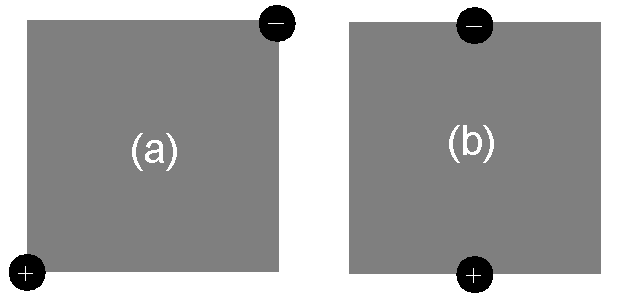
\includegraphics[scale=0.44]{2020-v3g-10-yl.pdf}
  \end{center}
  \vspace{-25pt}
\end{wrapfigure}
Ühtlase takistusega ruudust plaadi vastastippude vaheliseks takistuseks mõõdetakse
$R$, vt joonis (a). Milline tulemus saadakse sama ruudu vastaskülgede keskpunktide
vahelise takistuse mõõtmisel, vt joonis (b)? Mõlemal juhul kasutatakse oommeetri
ühendamiseks samu kettakujulisi tühise takistusega elektroode, mis surutakse vastu
plaati nii nagu näidatud joonisel.


\hint

\solu
Olgu $M$ ja $N$ vastavalt $AB$ ja $CD$ keskpunktid. Superpositsioneerime
ruudu, kus pinge on rakendatud $A$ ja $C$ vahele, ruuduga, kus pinge on
rakendatud $B$ ja $D$ vahele. Nüüd sümmeetria tõttu telge $MN$ ei läbi vool
ehk takistus $A$ ja $D$ vahel ristkülikus $AMND$ on samuti $R$. Peegeldame
$MN$ üle $AD$. Saame ruudu $M'MNN'$, külgede keskpunktidega $A$ ja $D$. $A$ ja
$D$ vaheline takistus sellises ruudus on kaks korda väiksem ehk $R/2$.
\probend